\documentclass[11pt,a4paper]{article}

% --- Core Packages ---
\usepackage[utf8]{inputenc}
\usepackage[margin=1in]{geometry}
\usepackage{amsmath,amssymb,amsfonts,amsthm}
\usepackage{booktabs}
\usepackage{graphicx}
\graphicspath{{figures/}{paper/figures/}}
\usepackage{tabularx}
\usepackage{microtype}
\usepackage{xcolor}
\usepackage{hyperref}
\usepackage{cite}

\hypersetup{
    colorlinks=true,
    linkcolor=blue!70!black,
    citecolor=green!50!black,
    urlcolor=blue!80!black
}

\title{\textbf{KevRouter: Decision Model Cost-Aware Router}}
\author{Blake de Haas \\
\texttt{blakedehaas@github.com}
\and Abhinav Dugar \\
\texttt{dugarabhinav2001@gmail.com}
}
\date{\today}

\begin{document}

\maketitle

% ==============================================================================
% ABSTRACT
% ==============================================================================
\begin{abstract}
% TODO: Abstract to be written at completion of experimental evaluation.
\noindent\textit{[TODO: Abstract to be completed upon final benchmark convergence.]}
\end{abstract}

% ==============================================================================
% SECTION 1: INTRODUCTION
% ==============================================================================
\section{Introduction}
\label{sec:introduction}
% TODO: Introduction to be written at completion of the study.
\noindent\textit{[TODO: Introduction to be completed at project conclusion.]}

% ==============================================================================
% SECTION 2: RELATED WORK
% ==============================================================================
\section{Related Work}
\label{sec:related_work}
% TODO: Related Work to be added upon literature synthesis.
\noindent\textit{[TODO: Related Work reviewing LLM cascade routing, mixture-of-agents, and calibration.]}

% ==============================================================================
% SECTION 3: DATASET AND BENCHMARK SUITE
% ==============================================================================
\section{Dataset and Benchmark Suite}
\label{sec:dataset}

To train and rigorously evaluate autonomous routing policies across heterogeneous workloads, our corpus is curated from \textsc{LLMRouterBench}, comprising 12,444 multi-model evaluated instances spanning 10 established benchmarks. The dataset encompasses broad factual recall, multi-step competition mathematics, professional college-level reasoning, complex code generation, and interactive agentic environments.

\subsection{Benchmark Composition and Evaluation Regimes}
\label{subsec:benchmark_composition}

The benchmark suite is partitioned into two distinct evaluation regimes:
\begin{enumerate}
    \item \textbf{In-Distribution ($\mathcal{D}_{\text{ID}}$)}: 9 diverse benchmarks comprising 12,166 unique queries used for model fine-tuning, temperature calibration, hyperparameter optimization, and held-out in-distribution test evaluation.
    \item \textbf{Out-of-Distribution ($\mathcal{D}_{\text{OOD}}$)}: $\tau^2$-Bench (278 queries), held out entirely from training and validation to evaluate zero-shot transfer to multi-turn agentic tool-use environments.
\end{enumerate}

\begin{table}[ht]
\centering
\small
\caption{Benchmark composition, domain coverage, solvability rate, and stratified sample counts.}
\label{tab:benchmark_suite}
\resizebox{\textwidth}{!}{%
\begin{tabular}{llcrrrr}
\toprule
\textbf{Benchmark} & \textbf{Target Domain / Capability} & \textbf{Solvability} & \textbf{Train} & \textbf{Val} & \textbf{Test ID} & \textbf{Total} \\
\midrule
SimpleQA        & Open-Domain Factuality \& Short QA       & 84.3\% & 3,461 & 432 & 433 & 4,326 \\
MMLU-Pro        & College-Level Multi-Disciplinary Reasoning& 95.0\% & 2,400 & 300 & 299 & 2,999 \\
HLE             & Humanity's Last Exam (Frontier Multimodal)& 51.0\% & 1,728 & 218 & 212 & 2,158 \\
LiveCodeBench   & Algorithmic Problem Solving \& Coding     & 92.0\% &   845 & 105 & 105 & 1,055 \\
ArenaHard       & Multi-Turn Instruction Following          & 97.7\% &   600 &  76 &  73 &   749 \\
SWE-Bench       & End-to-End Repository Bug Resolution      & 64.4\% &   398 &  50 &  52 &   500 \\
GPQA            & Graduate-Level Biology, Physics, Chem     & 97.0\% &   159 &  18 &  21 &   198 \\
LiveMathBench   & Fresh Competition Mathematics             & 84.3\% &    97 &  11 &  13 &   121 \\
AIME            & Elite Olympiad Mathematics                & 96.7\% &    50 &   5 &   5 &    60 \\
\midrule
\textbf{In-Distribution} & \textbf{Combined Primary Benchmarks} & \textbf{82.0\%} & \textbf{9,738} & \textbf{1,215} & \textbf{1,213} & \textbf{12,166} \\
\midrule
$\tau^2$-Bench (\textit{OOD}) & Multi-Turn Airline/Retail Agentic Tool Use & 93.5\% & --- & --- & 278 & 278 \\
\bottomrule
\end{tabular}%
}
\end{table}

As summarized in Table~\ref{tab:benchmark_suite}, the benchmark suite exhibits high difficulty variance. Highly solvable benchmarks like ArenaHard (97.7\%) and AIME (96.7\%) provide large cost-arbitrage opportunities for lightweight models. Conversely, HLE (51.0\%) and SWE-Bench (64.4\%) represent frontier capability bottlenecks where cost-effective models fail and routing must escalate to high-capacity reasoning flagships.

\subsection{Candidate Model Pool (13-Class Action Space)}
\label{subsec:candidate_models}

The router's destination action space $\mathcal{M}$ contains $|\mathcal{M}| = 13$ contemporary foundation models. The candidate endpoints span an execution cost disparity exceeding $125\times$, ranging from \$0.002 to \$0.250 per query.

\begin{table}[ht]
\centering
\small
\caption{Candidate model pool, execution pricing ($c_m$), in-distribution standalone accuracy, and cost-optimal market share across the ground-truth dataset.}
\label{tab:candidate_models}
\resizebox{0.95\textwidth}{!}{%
\begin{tabular}{llccc}
\toprule
\textbf{Model ($m$)} & \textbf{Provider / Family} & \textbf{Price / Query ($c_m$)} & \textbf{ID Accuracy} & \textbf{Optimal Share} \\
\midrule
\texttt{deepseek-v3-0324}             & DeepSeek          & \$0.002 & 41.28\% &  8.86\% \\
\texttt{gpt-5-chat}                   & OpenAI            & \$0.002 & 46.76\% &  3.88\% \\
\texttt{deepseek-v3.1-terminus}       & DeepSeek          & \$0.004 & 43.49\% & 10.16\% \\
\texttt{qwen3-235b-a22b-2507}         & Alibaba Cloud     & \$0.007 & 53.30\% & \textbf{47.96\%} \\
\texttt{intern-s1}                    & OpenGVLab         & \$0.010 & 36.91\% &  2.00\% \\
\texttt{kimi-k2-0905}                 & Moonshot AI       & \$0.012 & 44.02\% &  4.59\% \\
\texttt{claude-sonnet-4}              & Anthropic         & \$0.016 & 37.74\% &  0.48\% \\
\texttt{gemini-2.5-flash}             & Google DeepMind   & \$0.020 & 42.68\% &  6.17\% \\
\texttt{qwen3-235b-a22b-thinking-2507}& Alibaba Cloud     & \$0.021 & 52.12\% &  4.58\% \\
\texttt{deepseek-r1-0528}             & DeepSeek          & \$0.050 & 47.33\% &  1.47\% \\
\texttt{glm-4.6}                      & Zhipu AI          & \$0.055 & 43.75\% &  1.59\% \\
\texttt{gpt-5}                        & OpenAI            & \$0.150 & 57.64\% &  5.33\% \\
\texttt{gemini-2.5-pro}               & Google DeepMind   & \$0.250 & \textbf{58.80\%} &  2.92\% \\
\bottomrule
\end{tabular}%
}
\end{table}

As reported in Table~\ref{tab:candidate_models}:
\begin{itemize}
    \item \textbf{Single Best Model}: \texttt{gemini-2.5-pro} achieves the highest individual accuracy across $\mathcal{D}_{\text{ID}}$ at 58.80\%, but incurs the highest unit cost (\$0.250/query).
    \item \textbf{Cheapest Baseline}: \texttt{deepseek-v3-0324} achieves 41.28\% accuracy at \$0.002/query (a 17.52\% accuracy gap).
    \item \textbf{Workhorse Foundation}: \texttt{qwen3-235b-a22b-2507} captures 47.96\% of all optimal ground-truth instances, serving as the dominant balance point between cost (\$0.007) and accuracy (53.30\%).
    \item \textbf{Theoretical Oracle (Cheapest-Correct)}: Directing each solvable query to its lowest-cost successful model achieves an aggregate accuracy of \textbf{81.97\%} at an average cost of only \textbf{\$0.0122 / query}---reducing expenditure by $20.5\times$ compared to the flagship baseline while simultaneously improving task accuracy by +23.17\%.
\end{itemize}

\subsection{Ground-Truth Label Formulation}
\label{subsec:label_formulation}

For each query instance $x_i$, upstream execution logs record the binary task correctness $y_{i,m} \in \{0, 1\}$ and execution cost $c_{i,m}$ across all models $m \in \mathcal{M}$.

\paragraph{Deterministic Optimal Model ($m^*_i$)}
The primary hard label represents the cheapest model that correctly solves $x_i$:
\begin{equation}
m^*_i = \arg\min_{m \in \mathcal{M}_{\text{correct}}(x_i)} c_{i,m}, \quad \text{where} \quad \mathcal{M}_{\text{correct}}(x_i) = \{m \in \mathcal{M} \mid y_{i,m} = 1\}.
\end{equation}
If all 13 models fail on $x_i$ ($\mathcal{M}_{\text{correct}} = \emptyset$, representing 18.03\% of in-distribution instances), the label defaults to the lowest-cost model (\texttt{deepseek-v3-0324}), teaching the policy to avoid squandering expensive compute on unsolvable inputs.

\paragraph{Cost-Sensitive Soft Target Distribution ($q_i$)}
Because multiple models frequently solve a query with negligible price differences, training strictly against a one-hot label introduces artificial gradient penalties. We construct an exponential cost-discounted soft probability target distribution:
\begin{equation}
q(m \mid x_i) = \begin{cases} 
\frac{\exp\left(-\beta \cdot (c_{i,m} - c_{i,m^*})\right)}{\sum_{m' \in \mathcal{M}_{\text{correct}}(x_i)} \exp\left(-\beta \cdot (c_{i,m'} - c_{i,m^*})\right)}, & \text{if } m \in \mathcal{M}_{\text{correct}}(x_i), \\
0, & \text{if } m \notin \mathcal{M}_{\text{correct}}(x_i),
\end{cases}
\end{equation}
where $\beta = 20.0$ modulates the cost penalty steepness, concentrating mass on the cheapest correct candidates while softly crediting near-optimal alternatives.

\subsection{Hierarchical Doubly Stratified Partitioning}
\label{subsec:stratification}

To prevent covariate shift and preserve identical domain and difficulty distributions across partitions, we implement a \textbf{Hierarchical Doubly Stratified Sampling Strategy} (seed = 42).

Rather than stratifying over a single attribute, the corpus is partitioned across the joint distribution of \textbf{Benchmark Domain $\times$ Target Model Class} ($D \times M$):
\begin{enumerate}
    \item \textbf{Primary Stratum}: The dataset is segregated by benchmark dataset $D$ (AIME, GPQA, SWE-Bench, etc.).
    \item \textbf{Secondary Stratum}: Within each benchmark $D$, queries are partitioned into 13 bins by their optimal routing target $m^*$.
    \item \textbf{Deterministic Shuffling}: To ensure cross-platform reproducibility against non-deterministic filesystem orderings, records within each $(D, m^*)$ cell are sorted by the SHA-256 hash of their whitespace-normalized prompt text:
    \begin{equation}
    h_i = \text{SHA-256}(\text{normalize}(x_i)),
    \end{equation}
    and then pseudorandomly shuffled with seed 42.
    \item \textbf{Split Allocation}: Each cell is partitioned 80.0\% to Train (9,738 queries), 10.0\% to Validation (1,215 queries), and 10.0\% to In-Distribution Test (1,213 queries).
\end{enumerate}
This ensures that every individual benchmark maintains an exact 80/10/10 distribution, and every candidate model's target frequency is preserved without class starvation in small benchmarks.

\subsection{Validation Sub-Partitioning and Leakage Mitigation}
\label{subsec:validation_partitioning}

The 10\% validation split ($\mathcal{D}_{\text{val}}$, 1,215 queries) is subdivided into two statistically disjoint sets:
\begin{itemize}
    \item \textbf{Calibration Set ($N = 500$)}: Dedicated exclusively to post-hoc temperature scaling via Negative Log-Likelihood (NLL) minimization. Because temperature scaling optimizes a single 1D scalar parameter ($T \in \mathbb{R}^+$), 500 instances provide sufficient statistical power for convergence.
    \item \textbf{Development Set ($N = 715$)}: Dedicated to evaluating calibrated probabilities, conducting hyperparameter sweeps over loss weighting ($\mu$), and tuning confidence cascading thresholds ($\tau$).
\end{itemize}
\paragraph{Mitigation of Circular Validation Leakage}
Fitting temperature $T$ on the same validation samples used to evaluate calibration metrics (ECE, Brier score) or tune decision thresholds introduces circular selection bias: the temperature memorizes the sample residuals, yielding artificially optimistic calibration estimates. Maintaining strictly disjoint calibration and development sets guarantees that decision thresholds are tuned on genuinely unobserved probabilistic predictions.

\subsection{Prompt Length Distribution and 95th-Percentile Truncation}
\label{subsec:token_truncation}

Prompt lengths across the raw corpus exhibit extreme variance, spanning from 5 tokens up to 261,898 tokens (measured via Byte-Pair Encoding with \texttt{cl100k\_base}).

\begin{table}[ht]
\centering
\small
\caption{Empirical prompt length distribution across benchmarks (BPE tokens).}
\label{tab:length_distribution}
\resizebox{\textwidth}{!}{%
\begin{tabular}{lrrrrrr}
\toprule
\textbf{Benchmark} & \textbf{p50 (Median)} & \textbf{p75} & \textbf{p90} & \textbf{p95} & \textbf{p99} & \textbf{Max} \\
\midrule
SimpleQA        & 21 & 26 & 34 & \textbf{40} & 54 & 105 \\
LiveMathBench   & 119 & 150 & 192 & \textbf{221} & 263 & 366 \\
AIME            & 150 & 184 & 258 & \textbf{280} & 340 & 398 \\
$\tau^2$-Bench (\textit{OOD}) & 158 & 257 & 318 & \textbf{319} & 320 & 367 \\
MMLU-Pro        & 197 & 273 & 382 & \textbf{462} & 643 & 1,265 \\
GPQA            & 218 & 282 & 366 & \textbf{462} & 789 & 2,809 \\
HLE             & 183 & 316 & 555 & \textbf{847} & 1,740 & 13,560 \\
LiveCodeBench   & 526 & 667 & 814 & \textbf{942} & 1,209 & 1,639 \\
ArenaHard       & 90 & 267 & 733 & \textbf{1,391} & 3,223 & 7,406 \\
SWE-Bench       & 11,405 & 21,869 & 30,715 & \textbf{46,665} & 104,232 & 261,898 \\
\midrule
\textbf{In-Distribution ($\mathcal{D}_{\text{ID}}$)} & \textbf{136} & \textbf{287} & \textbf{604} & \textbf{1,219} & \textbf{22,117} & \textbf{261,898} \\
\bottomrule
\end{tabular}%
}
\end{table}

\paragraph{Informed Truncation Policy (1,024 Tokens)}
As detailed in Table~\ref{tab:length_distribution}, the empirical 95th percentile across all in-distribution queries is 1,219 tokens. Default short-text heuristics (e.g., 1,400 characters / $\approx 320$ tokens) severed 18.96\% of all instances, truncating essential function signatures in LiveCodeBench and problem descriptions in SWE-Bench.

We institute an empirical truncation threshold of \textbf{1,024 tokens} ($\approx 4,000$ characters):
\begin{itemize}
    \item Exactly \textbf{94.58\% of all in-distribution queries} (and 95.2\% of the training split) are retained completely losslessly with zero truncation.
    \item 100\% of SimpleQA, LiveMathBench, AIME, GPQA, $\tau^2$-Bench, and MMLU-Pro queries remain intact.
    \item For long-tail outliers (SWE-Bench), the initial 1,024 tokens capture the full issue statement, expected behavior, and reproduction stack trace, while pruning multi-megabyte git patch diffs that would otherwise induce quadratic attention memory blowup during routing.
\end{itemize}

\subsection{Dynamic Candidate Logit Masking}
\label{subsec:candidate_masking}

In the upstream release of $\tau^2$-Bench, \texttt{gpt-5-chat} was omitted from evaluation. Rather than discarding the benchmark or altering the 13-class routing space, we implement \textbf{Dynamic Candidate Logit Masking} at inference time:
\begin{equation}
z'_m(x) = \begin{cases} 
z_m(x), & \text{if } m \in \mathcal{M}_{\text{evaluated}}(x), \\ 
-\infty, & \text{if } m \notin \mathcal{M}_{\text{evaluated}}(x). 
\end{cases}
\end{equation}
Applying this mask prior to softmax normalization guarantees that unevaluated models receive zero probability mass, eliminating false-failure evaluation penalties while preserving architectural consistency.

% ==============================================================================
% SECTION 4: METHODS (FINE-TUNING METHODOLOGY)
% ==============================================================================
\section{Methods: Fine-Tuning Methodology}
\label{sec:methods}

KevRouter frames cost-aware routing as a learned single-pass decision model. Rather than generating free-form routing text or running multi-agent debate loops, the router predicts a calibrated probability distribution over destination endpoints in a single forward pass.

\subsection{Model Architecture: Backbone and PointerHead}
\label{subsec:architecture}

The routing architecture comprises an open foundation transformer backbone (Qwen 2.5 / 3.5 architecture) augmented with a lightweight, multi-option \textsc{PointerHead} decision mechanism.

\paragraph{Input Formulation}
Given a query $x$, the input sequence is formatted into a state context followed by structured option tokens describing the 13 candidate models and their routing criteria:
\begin{equation}
S = [\text{State: } x \ ; \ \text{Options: } \langle\text{opt}_1\rangle, \dots, \langle\text{opt}_K\rangle \ ; \ \langle\text{decide}\rangle].
\end{equation}

\paragraph{PointerHead Mechanism}
Let $h_{\text{decide}} \in \mathbb{R}^d$ denote the transformer hidden state corresponding to the final $\langle\text{decide}\rangle$ token, and let $H_{\text{opts}} \in \mathbb{R}^{K \times d}$ denote the hidden states pooled at each candidate option boundary $\langle\text{opt}_k\rangle$.

The PointerHead applies linear projections to map query decisions and option keys into a shared projection subspace of dimension $d_p = 256$:
\begin{align}
q &= W_q h_{\text{decide}} \in \mathbb{R}^{d_p}, \\
k_m &= W_k H_{\text{opts}}[m] \in \mathbb{R}^{d_p}, \quad \forall m \in \{1, \dots, K\},
\end{align}
where $W_q, W_k \in \mathbb{R}^{d_p \times d}$. The uncalibrated routing logit $z_m$ for candidate model $m$ is computed via scaled dot-product attention:
\begin{equation}
z_m = \frac{k_m^\top q}{\sqrt{d_p}}.
\end{equation}

\subsection{Parameter-Efficient Fine-Tuning (PEFT) via LoRA}
\label{subsec:peft_lora}

To enable parameter efficiency and prevent catastrophic forgetting of general semantic representations, the transformer backbone is adapted using Low-Rank Adaptation (LoRA).

For each targeted weight matrix $W_0 \in \mathbb{R}^{d_1 \times d_2}$, the weight update is decomposed into low-rank matrices $B \in \mathbb{R}^{d_1 \times r}$ and $A \in \mathbb{R}^{r \times d_2}$:
\begin{equation}
W = W_0 + \frac{\alpha}{r} B A,
\end{equation}
where $r = 16$ is the intrinsic adapter rank, $\alpha = 32$ is the scaling factor, and adapter dropout is set to $p_{\text{drop}} = 0.05$.

LoRA adapters are injected into:
\begin{itemize}
    \item Attention projection layers: Query ($W_q$), Key ($W_k$), Value ($W_v$), and Output ($W_o$).
    \item Multi-Layer Perceptron (MLP) layers: Gate ($W_{\text{gate}}$), Up-projection ($W_{\text{up}}$), and Down-projection ($W_{\text{down}}$).
\end{itemize}
The original backbone weights $W_0$ remain frozen. The trainable parameters consist solely of the LoRA matrices $\{A, B\}$ and the PointerHead projection weights $\{W_q, W_k\}$, representing less than 1.5\% of the total backbone parameter count.

\subsection{Training Objective}
\label{subsec:training_objective}

The model is trained on $\mathcal{D}_{\text{train}}$ using a cost-sensitive soft cross-entropy objective against the target distribution $q(m \mid x_i)$ defined in Section~\ref{subsec:label_formulation}:
\begin{equation}
\mathcal{L}_{\text{route}} = -\sum_{i=1}^{N} \sum_{m=1}^{|\mathcal{M}|} q(m \mid x_i) \log \left( \frac{\exp(z_{i,m})}{\sum_{j=1}^{|\mathcal{M}|} \exp(z_{i,j})} \right).
\end{equation}
Minimizing $\mathcal{L}_{\text{route}}$ is equivalent to minimizing the Kullback-Leibler (KL) divergence $\mathbb{D}_{\text{KL}}(q_i \parallel p_i)$ between the empirical cost-sensitive target distribution and the model's predicted softmax distribution.

The 4B and 9B experiments use AdamW with weight decay 0.01 and a one-cycle learning-rate schedule. Two configurations were evaluated: one epoch at learning rate $2 \times 10^{-5}$ and three epochs at $2 \times 10^{-4}$. Because both settings differ, their comparison does not isolate epoch count. The historical 0.8B results use one epoch; the exact training-record manifest is unavailable.

\subsection{Post-Hoc Probability Calibration}
\label{subsec:calibration_method}

Following training, the model's logits are calibrated using temperature scaling on the held-out calibration partition ($\mathcal{D}_{\text{cal}}$, $N = 500$):
\begin{equation}
\hat{p}_m(x) = \frac{\exp(z_m / T)}{\sum_{j=1}^{|\mathcal{M}|} \exp(z_j / T)},
\end{equation}
where the scalar temperature $T > 0$ is obtained by minimizing Negative Log-Likelihood via L-BFGS:
\begin{equation}
T^* = \arg\min_{T > 0} \left[ - \sum_{i \in \mathcal{D}_{\text{cal}}} \sum_{m=1}^{|\mathcal{M}|} q(m \mid x_i) \log \left( \frac{\exp(z_{i,m} / T)}{\sum_{j=1}^{|\mathcal{M}|} \exp(z_{i,j} / T)} \right) \right].
\end{equation}
The optimal temperature $T^*$ is frozen into the deployed decision head, producing well-calibrated confidence scores.

\subsection{Inference-Time Decision Rules}
\label{subsec:decision_rules}

Given calibrated probabilities $\hat{p} \in \Delta^{|\mathcal{M}|-1}$ and known model pricing vectors $c \in \mathbb{R}^{|\mathcal{M}|}$, the router executes one of three decision policies:

\paragraph{1. Greedy Argmax Policy}
Directs the query to the endpoint with the highest estimated success probability:
\begin{equation}
m^*_{\text{argmax}} = \arg\max_{m \in \mathcal{M}} \hat{p}_m(x).
\end{equation}

\paragraph{2. Gentle Utility Cost-Penalized Policy}
Penalizes expensive endpoints by trading marginal confidence against execution cost via regularizer $\mu \ge 0$:
\begin{equation}
m^*_{\text{utility}} = \arg\max_{m \in \mathcal{M}} \left[ \hat{p}_m(x) - \mu \cdot c_m \right].
\end{equation}
Varying $\mu$ shifts routing mass according to the probability and fixed model cost proxies. For the 4B and 9B analysis, we sweep 503 values from zero through 100 on $\mathcal{D}_{\text{dev}}$ and select settings under prespecified average-cost budgets.

\paragraph{3. Confidence-Gated Cascading Policy}
Partitions $\mathcal{M}$ into a cost-effective tier $\mathcal{M}_{\text{cheap}}$ ($c_m \le \$0.010$) and a frontier flagship tier $\mathcal{M}_{\text{flagship}}$. The router evaluates whether the top cost-effective candidate meets confidence threshold $\tau \in [0.60, 0.85]$:
\begin{equation}
m^*_{\text{cascade}} = \begin{cases} 
\arg\max_{m \in \mathcal{M}_{\text{cheap}}} \hat{p}_m(x), & \text{if } \max_{m \in \mathcal{M}_{\text{cheap}}} \hat{p}_m(x) \ge \tau, \\
\arg\max_{m \in \mathcal{M}_{\text{flagship}}} \hat{p}_m(x), & \text{otherwise.}
\end{cases}
\end{equation}
This rule does not guarantee accuracy preservation; its empirical accuracy and cost are evaluated below.

% ==============================================================================
% SECTION 5: EXPERIMENTS AND RESULTS
% ==============================================================================
\section{Experiments and Results}
\label{sec:experiments}

We evaluate KevRouter on the full LLMRouterBench suite across in-distribution and out-of-distribution benchmarks. In accordance with the evaluation hierarchy established in Section~\ref{sec:methods}, our analysis prioritizes:
\begin{enumerate}
    \item \textbf{Routing Accuracy (\%):} Proportion of queries routed to an endpoint that produces a fully correct response ($\text{score} \ge 1.0$).
    \item \textbf{Optimal Match Rate (\%):} Proportion of queries routed specifically to the Pareto-optimal (cheapest correct) model.
    \item \textbf{Cost per Correct Answer (\$/query):} Total expenditure incurred divided by the number of correct responses, measuring net economic efficiency.
    \item \textbf{Routing Latency (ms):} Single-pass forward runtime on the local host.
\end{enumerate}

\subsection{Experimental Setup}
\label{subsec:exp_setup}

The historical 0.8B model was trained and evaluated on an NVIDIA GeForce RTX 5080 (16GB VRAM, CUDA 13.5). The router utilizes the open 852M parameter \texttt{Qwen/Qwen3.5-0.8B-Base} architecture with low-rank adaptation ($r=16, \alpha=32$) and PointerHead projection ($d_p=256$), comprising 11.3M trainable parameters. Training executes for one complete epoch over 9,193 admitted training records in \texttt{bfloat16} with gradient checkpointing, batch size 1, and 8 accumulation micro-batches (effective batch size 8). Total fine-tuning runtime was 104.97 minutes with peak VRAM utilization of 3.92 GB.

For the historical 0.8B run, the paper reports a fitted temperature $T^* = 0.6156$ (Brier score: 0.7149, ECE: 0.3066). The 4B and 9B experiments and their calibration procedures are described separately below. The original 0.8B record-level predictions and training manifest are unavailable for independent verification.

\subsection{Comparative Benchmark Matrix}
\label{subsec:benchmark_matrix}

Table~\ref{tab:results_matrix} reports the comprehensive performance comparison between the zero-shot base checkpoint (\textsc{Kev-0.8B Base}) and fine-tuned KevRouter under three inference decision rules: greedy calibrated ArgMax, Cost-Utility Bayes optimization ($\mu=2.5$), and confidence-gated cascading ($\tau=0.6$).

\begin{table}[t]
\centering
\small
\caption{Comprehensive performance matrix across validation, held-out in-distribution test, and out-of-distribution ($\tau^2$-Bench) splits on LLMRouterBench. Best results per metric within each split are bolded.}
\label{tab:results_matrix}
\resizebox{\textwidth}{!}{%
\begin{tabular}{llrrrrr}
\toprule
\textbf{Model} & \textbf{Decision Policy} & \textbf{Accuracy} & \textbf{Optimal} & \textbf{Avg Cost} & \textbf{Cost / Correct} & \textbf{Latency} \\
 & & \textbf{(\%)} & \textbf{(\%)} & \textbf{(\$/query)} & \textbf{(\$/correct)} & \textbf{(ms)} \\
\midrule
\multicolumn{7}{l}{\textbf{Validation Split} ($\mathcal{D}_{\text{val}}$, $N=1,215$)} \\
Kev-0.8B (Base)       & ArgMax (Zero-Shot)       & 47.49\% &  3.46\% & \$0.00712 & \$0.01499 & 91.5 \\
Kev-0.8B (Fine-Tuned) & Calibrated ArgMax        & \textbf{59.42\%} & \textbf{39.01\%} & \$0.01577 & \$0.02654 & 90.8 \\
Kev-0.8B (Fine-Tuned) & Cost-Utility ($\mu=2.5$)  & 54.07\% & 36.38\% & \textbf{\$0.00098} & \textbf{\$0.00181} & 90.8 \\
Kev-0.8B (Fine-Tuned) & Cascading ($\tau=0.6$)   & \textbf{59.42\%} & \textbf{39.01\%} & \$0.01577 & \$0.02654 & 90.8 \\
\midrule
\multicolumn{7}{l}{\textbf{Held-Out In-Distribution Test Split} ($\mathcal{D}_{\text{test-ID}}$, $N=1,213$)} \\
Kev-0.8B (Base)       & ArgMax (Zero-Shot)       & 45.75\% &  3.63\% & \$0.00765 & \$0.01672 & 92.9 \\
Kev-0.8B (Fine-Tuned) & Calibrated ArgMax        & \textbf{56.72\%} & \textbf{36.44\%} & \$0.01447 & \$0.02551 & 98.9 \\
Kev-0.8B (Fine-Tuned) & Cost-Utility ($\mu=2.5$)  & 53.09\% & 35.28\% & \textbf{\$0.00087} & \textbf{\$0.00164} & 98.9 \\
Kev-0.8B (Fine-Tuned) & Cascading ($\tau=0.6$)   & \textbf{56.72\%} & \textbf{36.44\%} & \$0.01447 & \$0.02551 & 98.9 \\
\midrule
\multicolumn{7}{l}{\textbf{Out-of-Distribution Transfer Split} ($\tau^2$-Bench, $N=278$)} \\
Kev-0.8B (Base)       & ArgMax (Zero-Shot)       & 15.47\% &  2.88\% & \$0.06859 & \$0.44341 & \textbf{90.9} \\
Kev-0.8B (Fine-Tuned) & Calibrated ArgMax        & \textbf{40.29\%} & \textbf{25.18\%} & \textbf{\$0.04198} & \textbf{\$0.10421} & 95.7 \\
Kev-0.8B (Fine-Tuned) & Cost-Utility ($\mu=2.5$)  & \textbf{40.29\%} & \textbf{25.18\%} & \textbf{\$0.04198} & \textbf{\$0.10421} & 95.7 \\
Kev-0.8B (Fine-Tuned) & Cascading ($\tau=0.6$)   & \textbf{40.29\%} & \textbf{25.18\%} & \textbf{\$0.04198} & \textbf{\$0.10421} & 95.7 \\
\bottomrule
\end{tabular}%
}
\end{table}

\subsection{4B and 9B Experiments}
\label{subsec:larger_models}

We additionally evaluated pretrained Kev 4B and 9B checkpoints and fine-tuned each on LLMRouterBench using rank-16 LoRA and the trainable routing head on an NVIDIA A100 80GB GPU. The Qwen backbones remained frozen. One run per model used one epoch at $2\times10^{-5}$; a second used three epochs at $2\times10^{-4}$, with batch size one and gradient accumulation over eight records. Both configurations admitted 9,193 training records under the same Qwen-tokenizer context filter used by the current pipeline: 545 of 9,738 records were excluded, including all 398 SWE-Bench records. This matches the reported 0.8B count, but the historical record-level manifest is unavailable, so exact identity cannot be verified. The three-epoch jobs each completed in approximately 9 hours 40 minutes including calibration and evaluation.

The one-epoch runs fitted temperature against hard labels using the installed trainer's grid search; the three-epoch runs fitted temperature on 500 held-out calibration examples by minimizing soft-target negative log-likelihood with L-BFGS-B. A positive temperature does not alter the argmax ordering. For the three-epoch runs, calibrated probabilities support the cost and tier policies below. Each development and test evaluation scores only candidates with a recorded outcome; on OOD, this excludes \texttt{gpt-5-chat}. Such offline masking is not a guarantee of deployment-time availability. Routing accuracy is the fraction of queries for which the selected candidate has recorded score at least one; cost is the recorded downstream cost and excludes router inference cost.

\begin{table}[t]
\centering
\small
\caption{Argmax results for historical 0.8B runs and the new 4B and 9B runs, compared with selecting Qwen 235B for every query. ID has 1,213 records and OOD has 278. Cost is the mean recorded ID downstream cost per query. The 0.8B rows are reported historical aggregates, without record-level predictions available for verification.}
\label{tab:size_results}
\begin{tabular}{lrrr}
\toprule
\textbf{Router / policy} & \textbf{ID accuracy} & \textbf{OOD accuracy} & \textbf{ID cost} \\
\midrule
0.8B pretrained (historical) & 45.75\% & 15.47\% & \$0.00765 \\
0.8B fine-tuned, 1 epoch (historical) & 56.72\% & 40.29\% & \$0.01447 \\
4B pretrained & 43.61\% & 41.01\% & \$0.00801 \\
4B fine-tuned, 1 epoch & 56.64\% & 40.29\% & \$0.01464 \\
4B fine-tuned, 3 epochs & 56.14\% & 37.77\% & \$0.01118 \\
9B pretrained & 45.01\% & 9.71\% & \$0.00959 \\
9B fine-tuned, 1 epoch & 56.80\% & 40.29\% & \$0.01421 \\
9B fine-tuned, 3 epochs & 56.31\% & 38.13\% & \$0.01115 \\
Fixed Qwen 235B & 53.42\% & 40.29\% & \$0.00083 \\
\bottomrule
\end{tabular}
\end{table}

Table~\ref{tab:size_results} shows a substantial ID improvement from fine-tuning each larger router, but no clear accuracy advantage from increasing router size. The three-epoch 4B and 9B models chose different destinations on 519 of 1,213 ID records; 4B alone was correct on 66 and 9B alone on 68. Their similar aggregate accuracy therefore does not imply identical routing behavior. On OOD, the one-epoch 4B and 9B models chose Qwen 235B on all 278 records, explaining their identical 40.29\% accuracy.

\subsection{Development-Selected Cost Policies}
\label{subsec:cost_curves}

Using saved calibrated probabilities from the three-epoch runs, we swept 503 values of $\mu$: zero, a logarithmic grid from $10^{-4}$ to 100, and 2.5. For each router and each prespecified development average-cost budget of \$0.001, \$0.002, \$0.005, \$0.010 and \$0.020 per query, we selected the highest-accuracy eligible setting on the 715-record development set, breaking ties by lower cost and then lower $\mu$. The fixed model cost proxies in the decision rule differ from the per-query recorded costs used to evaluate mean expenditure. An empirical budget on development is not a per-query guarantee and need not hold on other distributions. ID and OOD results had already been inspected before this analysis and are not fresh confirmation sets.

\begin{table}[t]
\centering
\small
\caption{Development-selected cost-utility policies evaluated on the ID test set. Budgets refer to development mean cost, not test-time guarantees. All costs exclude router inference.}
\label{tab:cost_sweep}
\begin{tabular}{lrrrr}
\toprule
\textbf{Router} & \textbf{Dev. budget} & $\boldsymbol{\mu}$ & \textbf{ID accuracy} & \textbf{ID cost} \\
\midrule
4B & \$0.001 & 73.7904 & 46.74\% & \$0.00089 \\
4B & \$0.002 & 15.2757 & 48.39\% & \$0.00152 \\
4B & \$0.005 & 0.7516 & 53.83\% & \$0.00475 \\
4B & \$0.010 & 0.0871 & 54.66\% & \$0.00901 \\
4B & \$0.020 & 0.0000 & 56.14\% & \$0.01118 \\
9B & \$0.001 & 73.7904 & 46.08\% & \$0.00092 \\
9B & \$0.002 & 1.5849 & 53.34\% & \$0.00184 \\
9B & \$0.005 & 1.2706 & 53.83\% & \$0.00239 \\
9B & \$0.010 & 0.1117 & 55.32\% & \$0.00940 \\
9B & \$0.020 & 0.0023 & 56.39\% & \$0.01114 \\
\midrule
Fixed Qwen 235B & --- & --- & 53.42\% & \$0.00083 \\
Fixed GPT-5 & --- & --- & 56.55\% & \$0.02933 \\
Fixed Gemini 2.5 Pro & --- & --- & 58.37\% & \$0.06039 \\
\bottomrule
\end{tabular}
\end{table}

\begin{figure}[t]
\centering
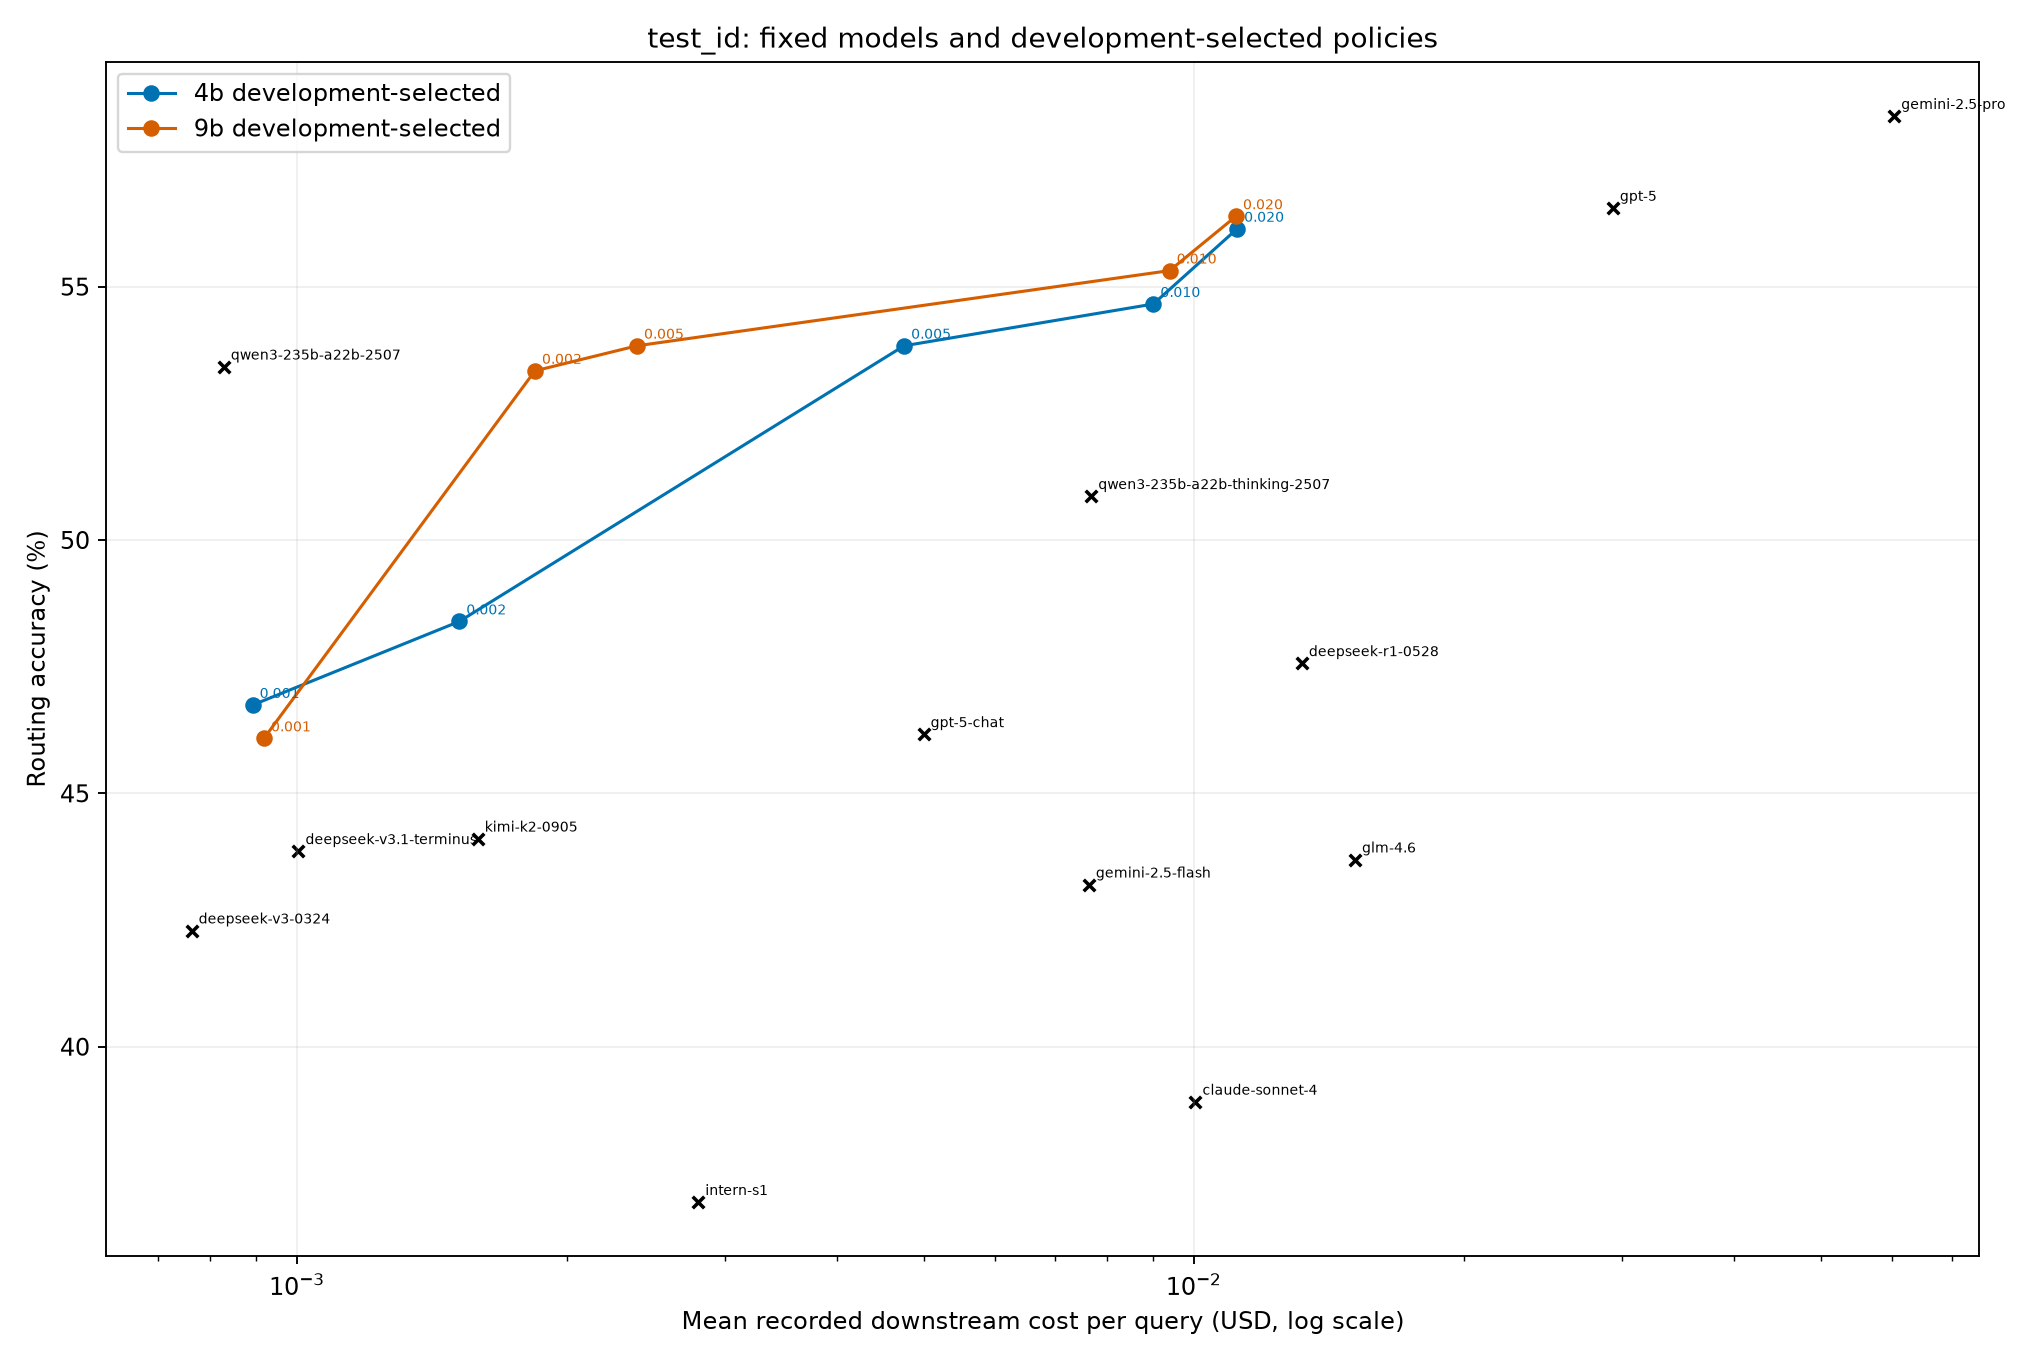
\includegraphics[width=\textwidth]{figures/kev_id_accuracy_cost.png}
\caption{ID test accuracy and recorded downstream cost for every fixed-model baseline and the 4B/9B policies selected on development. Labels on router points denote development budgets in dollars per query. Lines connect evaluated settings and do not establish performance at interpolated points.}
\label{fig:id_cost}
\end{figure}

At the \$0.005 development budget, the selected 9B policy reached 53.83\% ID accuracy at \$0.00239 per query, compared with 53.42\% at \$0.00083 for fixed Qwen. The 9B argmax policy reached 56.31\% at \$0.01115. Figure~\ref{fig:id_cost} places these operating points alongside all 13 fixed candidates; no single claim of cost efficiency applies independently of the desired accuracy and baseline.

\subsection{Paired Uncertainty and Error Analysis}
\label{subsec:paired_uncertainty}

We computed paired 95\% percentile bootstrap intervals from 5,000 resamples, clustering on query hash and using the same sampled clusters for both methods. Intervals describe sampling variation conditional on the saved trained models, not retraining variance or multiple-comparison uncertainty. For ID, three-epoch 9B argmax minus fixed Qwen was $+2.89$ percentage points (95\% interval $[+0.66,+5.11]$): 9B alone succeeded on 112 records and Qwen alone on 77. For the 9B policy selected at the \$0.005 development budget, the difference was $+0.41$ points ($[-1.57,+2.39]$), with 80 and 75 unique successes respectively. Three-epoch 4B minus 9B argmax was $-0.16$ points ($[-2.06,+1.65]$). The one-epoch 4B minus 9B interval was $[-0.99,+0.66]$ points. The historical 0.8B aggregate lacks per-record predictions and cannot be included in paired comparisons.

Comparing three-epoch 9B argmax with fixed Qwen, ID correct counts were 32 versus 20 of 212 HLE records and 81 versus 72 of 105 LiveCodeBench records. They were 239 versus 240 of 299 MMLU-Pro records and 11 versus 11 of 52 SWE-Bench records. The three-epoch 9B router selected GPT-5 for 180 ID records, accounting for \$9.47 of its \$13.53 total recorded downstream cost; GPT-5 answered 69 of those selected records correctly. These queries are selected by the router and need not have the same difficulty as other queries. Breakdown by prompt length is similarly descriptive because length and benchmark type are correlated. Small per-benchmark groups and repeated inspection warrant caution.

\subsection{Exploratory OOD Comparison}
\label{subsec:ood_baselines}

OOD contains 278 records with 167 distinct query hashes; bootstrap resampling clusters repeated query text, which may occur in distinct scenarios. The three-epoch 4B tier gate at $\tau=0.6$ achieved 48.92\% at \$0.10027 per query while selecting \texttt{kimi-k2-0905} on 273 records. Fixed Kimi achieved the same 48.92\% at \$0.10036. Fixed \texttt{glm-4.6} achieved 53.96\% at \$0.09931, exceeding the gate's observed accuracy at lower recorded cost. Thus, improvement over fixed Qwen alone is insufficient to establish an OOD routing benefit. Figure~\ref{fig:ood_cost} compares all 12 available OOD fixed candidates with the unchanged development-selected 4B and 9B policies. These post hoc OOD comparisons are exploratory.

\begin{figure}[t]
\centering
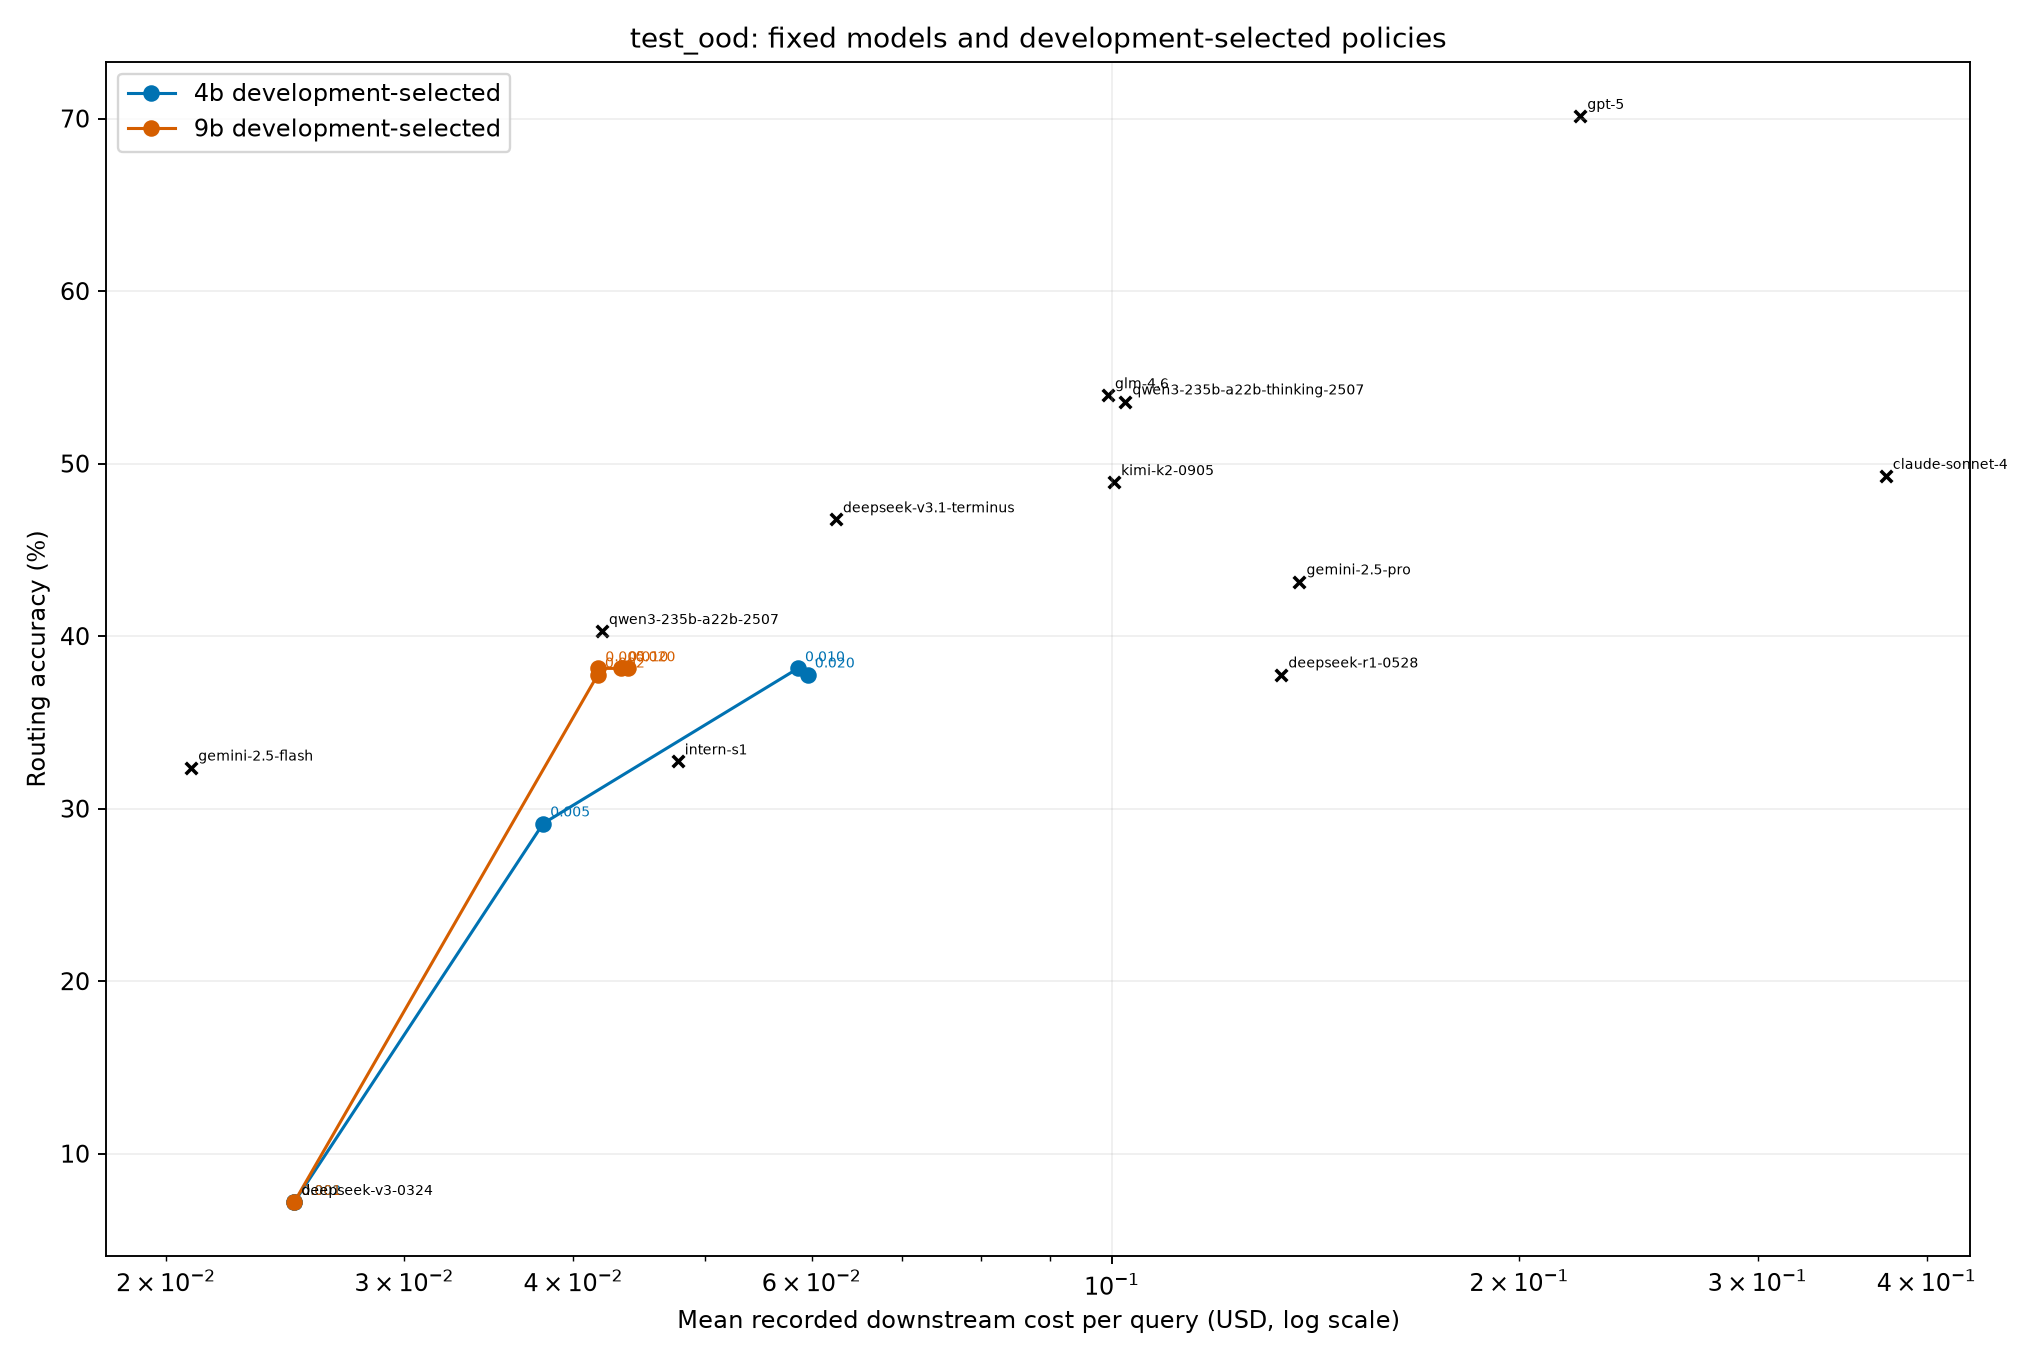
\includegraphics[width=\textwidth]{figures/kev_ood_accuracy_cost.png}
\caption{Exploratory OOD accuracy and recorded downstream cost for all available fixed models and the unchanged development-selected policies. Cost and accuracy reflect the benchmark's recorded outputs.}
\label{fig:ood_cost}
\end{figure}

% ==============================================================================
% SECTION 6: DISCUSSION
% ==============================================================================
\section{Discussion}
\label{sec:discussion}
Fine-tuning improves ID accuracy for both larger routers, but the observed 4B--9B difference is small and uncertain. The trade-off with fixed-model baselines is central: argmax routing improves ID accuracy over fixed Qwen at substantially greater recorded downstream cost, while the selected cheaper operating point does not establish an accuracy improvement. On OOD, the near-constant Kimi tier-gate choice illustrates why comparisons against several fixed candidates are necessary. The original 0.8B per-record outputs and exact training manifest are unavailable, the test sets have been examined repeatedly, and the two larger-model training configurations vary both epoch count and learning rate. These limitations prevent a controlled scaling or generalization claim.

% ==============================================================================
% SECTION 7: CONCLUSION
% ==============================================================================
\section{Conclusion}
\label{sec:conclusion}
On LLMRouterBench, fine-tuned 4B and 9B Kev routers achieve approximately 56--57\% ID argmax accuracy, close to the previously reported 0.8B result. The 9B router improves ID accuracy over always choosing Qwen in a paired analysis, but at considerably higher recorded downstream cost. Development-selected cost policies and OOD fixed-model comparisons show that a routing benefit depends on the operating point and baseline. Independent held-out evaluation and controlled training ablations are needed to assess stability and generalization.

\end{document}

